%% intro.tex
%% Copyright (C) 2014 by Thomas Auzinger <thomas.auzinger@cg.tuwien.ac.at>
%
% This work may be distributed and/or modified under the
% conditions of the LaTeX Project Public License, either version 1.3
% of this license or (at your option) any later version.
% The latest version of this license is in
%   http://www.latex-project.org/lppl.txt
% and version 1.3 or later is part of all distributions of LaTeX
% version 2005/12/01 or later.
%
% This work has the LPPL maintenance status `maintained'.
%
% The Current Maintainer of this work is Thomas Auzinger.
%
% This work consists of the files vutinfth.dtx and vutinfth.ins
% and the derived file vutinfth.cls.
% This work also consists of the file intro.tex.


\newacronym{ctan}{CTAN}{Comprehensive TeX Archive Network}
\newacronym{faq}{FAQ}{Frequently Asked Questions}
\newacronym{pdf}{PDF}{Portable Document Format}
\newacronym{svn}{SVN}{Subversion}
\newacronym{wysiwyg}{WYSIWYG}{What You See Is What You Get}

\newglossaryentry{texteditor}
{
  name={editor},
  description={A text editor is a type of program used for editing plain text files.}
}

In this chapter, we will present our integer programming formulation for shift design and break scheduling problems in details.  The integer programming approach is explained separately in two subsections. In each subsection, we describe the variables that we used, the constraints and the objective function. 

\section{Integer Linear Programming Model for Shift Design Problem}

The explicit set covering formulation have been first proposed for the shift scheduling problem by Dantzig (1954) \cite{li:1954:dantzig}. Our integer programming formulation is also based on an explicit representation of shift design. To formulate the shift design problem explicitly, we generate all shifts including all feasible combinations of shift start times and lengths. The model uses the following variables.

\subsection{Variables}

The variables of integer programming formulation consist of two parts, input and decision variables.

\subsubsection{Input Variables}

We presented the original problem definition in the second chapter, we will define the input and the generated variables from the given instance. For shift design problem formulation, the input variables are, \\

\begin{itemize}
\item $slotLength :$ All time slots have the same length of interval $slotLength$ and it is usually 15, 30 or 60 minutes for the shift design problem.

\item $daysPerCycle :$ The number of days in the planning period. $daysPerCycle$ is considered typically a week (7 days).
The shift design problem has a cyclic structure. Assuming 7 days of period, the last time slot $t_{n+1}$ of the seventh day is equal to the first time slot $t_1$ of the first day. 

\item $n :$ Number of consecutive time slots with same $slotLength$. The calculation of $n$ variable is,

\begin{equation}
 n = daysPerCycle * 24 *  60 / slotLength
\end{equation}

\item $m :$ Number of all enumerated possible shifts. All possible shifts are generated based on minimum / maximum shift starts and minimum / maximum shift lengths. The variable $m$ is calculated as follows ($y$ is defined in the problem statement chapter as the number of shift types),

\begin{equation}
m = \sum_{i=1}^y Distinct Start_i * Distinct Length_i
\end{equation}

Suppose that, we have given the shift types in Table~\ref{tab:shifttypes2}. Assuming a $slotLength$ of 60 minutes, morning shifts can start  05:00, 06:00, 07:00 or 08:00 and the length of shifts can be 7, 8 or 9 hours. The number of possible distinct shifts for the morning shift type is 12 (4 different starting hours * 3 different shift lengths). Further, there will be 9 possible shifts for the day, 9 for the afternoon and 9 for the night shifts. In total, the number of possible shifts including all feasible combinations of shift start times and lengths is 39, for the slotlength 60. 110 possible shifts for the slotlength 30 and 360 possible shifts for the $slotLength$ 15. \\

\begin{table}
  \centering
  \begin{tabular}{ccccc}
    \toprule
    Shift type & MinStart         & MaxStart      & MinLength & MaxLength        \\
    \midrule
    M     & 05:00	 & 08:00          & 07:00 	& 09:00        \\
    D     & 09:00	 & 11:00          & 07:00	& 09:00        \\
    A     & 13:00	 & 15:00          & 07:00	& 09:00        \\
    N     & 21:00	 & 23:00          & 07:00	& 09:00        \\
    \bottomrule
  \end{tabular}
  \caption{An example of shift types}
  \label{tab:shifttypes2} 
\end{table}

\item $x_t : $ Number of employees are needed for time slot $t$ (defined as variable $w_i$ in the original problem definition). 

\begin{equation}
x_t \ge 0 \quad \forall t = 1, 2, ..., n
\end{equation}

\item $a_{ts} :$ For each possible shift $s$, we set the $a_{ts}$ variable to 1, if time slot $t$ is in the working period of shift $s$, 0 otherwise.


\begin{equation}
a_{ts} = \left\{ \begin{array}{cc}
		1 & \mbox{if time slot t is a work period of shift s} \\
		0 & \mbox{otherwise}
	    \end{array}
    \right.
\end{equation}

\begin{equation}
a_{ts} \in \{0, 1\} \quad \forall t = 1, 2, ..., n  \quad \forall s = 1, 2, ..., m
\end{equation}

For instance, the first enumerated shift based on Table~\ref{tab:shifttypes}, will start at 05.00 and its length is 7 hours. All time slots $t$ between [05.00, 12.00) set to 1 in each day of the time period, likewise [12.00-05.00) must be equal to 0.


\item $W_i$ : Weight of the three component. 
\begin{equation}
W_i \ge 0 \quad \forall i = 1, 2, 3
\end{equation}
\end{itemize}

\subsubsection{Decision Variables}

Integer linear programming formulation for the shift design problem, the decision variables are given below,
\begin{itemize}
\item $b_s : $ For each enumerated shift, we use the variable $b_s$ indicating, whether shift is used or not. 

\begin{equation}
b_s  = \left\{ \begin{array}{cc}
		1 & \mbox{if the shift is active} \\
		0 & \mbox{otherwise}
	    \end{array}
    \right.
\end{equation}

 The variable $b_s$ is initialized in Cplex Solver as,

\begin{lstlisting}[frame=single, numbers=left]
b=cplex.numVarArray(m, 0, 1, IloNumVarType.Bool);
\end{lstlisting}

\item $w_{sd} : $ Number of employees, that are assigned to a shift $s$ during the day $d$. The same shifts can have different number of employees in different days. This integer programming variable has two dimensions, shift number and day number. The initialization of the number of workers $w_{sd}$ in Cplex Solver is illustrated below,

\begin{lstlisting}[frame=single, numbers=left]
w=new IloNumVar[m][]; 
for (int s = 0; s < m; s++){ 
	w[s]=cplex.numVarArray(daysPerCycle, 0, 
		Integer.MAX_VALUE, IloNumVarType.Int);				
}	
\end{lstlisting}

\item The three components of the objective function are :

\begin{itemize}
\item[] $F_0$ : Sum of the excesses of workers in each time slot. 

\item[] $F_1$ : Sum of the shortages of workers in each time slot.

\item[] $F_2$ : Number of shifts.
 \end{itemize}

We initialized these three components of the objective function as follows in Cplex Solver,

\begin{lstlisting}[frame=single, numbers=left]
F=cplex.numVarArray(3,0, Integer.MAX_VALUE, IloNumVarType.Int);
\end{lstlisting}

\item $l_t : $ The load for time slot $t$. The load $l_t$ represents the sum of the number of workers, who works in time slot $t$ in all shifts. The initialization of load $l_t$ in Cplex Solver is,

\begin{lstlisting}[frame=single, numbers=left]
l=cplex.numVarArray(n,0, Integer.MAX_VALUE, IloNumVarType.Int);
\end{lstlisting}


\item $ex_t : $ The excesses of workers for each time slot $t$.

\item $sh_t : $ The shortages of workers  for each time slot $t$.

We illustrate excesses $ex_t$ and shortages $sh_t $ of workers for each time slot in Cplex Solver below,
\begin{lstlisting}[frame=single, numbers=left]
ex=cplex.numVarArray(n,0,Integer.MAX_VALUE,IloNumVarType.Int);
sh=cplex.numVarArray(n,0,Integer.MAX_VALUE,IloNumVarType.Int);
\end{lstlisting}

We defined the variables, that we use in our integer programming model. In the next section, we will present the constraints.

\end{itemize}


\subsection{Constraints}
We will present the constraints, we use in our integer programming formulation in 2 sections based on the component of the objective function, excesses and shortages of workers in each time slot ($F_0, F_1 $) and number of shifts ($F_2$)

\subsubsection{Excesses and Shortages of Workers in each Time Slot ($F_0 , F_1 $)}
The shift scheduling problem focuses on minimum number of employees, without any shortages. On the other hand, in shift design problem, we need to consider not only over staffing, but also under staffing component in the objective function. In order to find the sum of excesses and shortages of employees, first we need to define the load $l_t$ variable of time slot $t$ as follows,

\begin{equation}
l_t = \sum_{s=1}^m (a_{ts} * w_{s,  (daysPerCycle * t  / n)}) \quad \forall t = 1,2 ...n
\end{equation}


The load $l_t$ of each time slot $t$ is the sum of employees for every possible shift work during this period. The variable $a_{ts}$ is used, whether the time slot $t$ is in the time window of the shift $s$. If $a_{ts}$ variable is equal to 1, the number of workers $w_{sd}$ of the shift $s$ on this day is added to the equation. The day number $d$ for the variable $w_{sd}$ from the time slot $t$  is calculated with the following equation, 

\begin{equation}
d = t/(24 * 60/slotlength)= daysPerCycle * t / n 
\end{equation}

There is one challenge to find the day number in $w_{sd}$ parameter from the time slot $t$. We need to consider the shifts, which start in one day $d$ and continuing into the following day $d+1$. $w_{sd}$ is the number of workers of shift $s$, which starts to their shift in day $d$. From the calculation above, we needed to update the day number of the time slot of the next day in variable $w_{sd}$ to the one day before. 

As an example, suppose we have 4 employees at one of the night shift on the first day  ($w_{s1} = 4 $) and in the same shift have 2 employees on the second day ($w_{s2} = 2 $). If we calculate with the formulation above the day value at 01.00 o'clock on the second day, the formula will find $w_{s2} = 2 $, $w_{s2}$ is the number of workers on shift $s$ on the second day. However, we need to use the number of employees on the first day, because the shift started on Monday. Due to this problem, $nextDay_s$ variable is used, whether the shift continues in time slot of the next day or not. In every shift, that has true value of $nextDay_s$ variable, then if the time slot $t$ is after midnight, the day number will be decreased one.



\begin{lstlisting}[frame=single, numbers=left]
IloLinearNumExpr[] expr2 = new IloLinearNumExpr[n];
for ( int t = 0; t < n; t++){
    expr2[t] = cplex.linearNumExpr();
    for ( int s = 0; s < m; s++){
        if(t % (24 * 60 / slotLength) < 12 * 60 / slotLength  
	&& nextDay[s] == true ){
            tempDay = ((daysPerCycle *t/n) + daysPerCycle -1) 
			% daysPerCycle;
        }
        else 
            tempDay = (daysPerCycle *t/n);
        expr2[t].addTerm(a[t][s], w[s][tempDay]);
    }
    cplex.addEq (l[t], expr2[t]);
}
\end{lstlisting}

From the formal definition of the shift design problem in \cite{li:2004:musliu}, the sum of excesses and shortages of workers is defined as follows,

\begin{equation}
F_0 = \sum_{t=1}^n \max (l_t - x_t, 0) * slotlength
\end{equation}
\begin{equation}
F_1 = \sum_{t=1}^n \max (x_t - l_t, 0) * slotlength
\end{equation}

Instead of using maximum operator in Cplex Solver, we calculate the excesses and shortages of workers in each time slot $t$,

\begin{equation}
ex_t \ge (l_t - x_t) * slotlength  \quad  \forall t = 1,2 ...n
\end{equation}
\begin{equation}
sh_t \ge (x_t - l_t) * slotlength \quad  \forall t = 1,2 ...n
\end{equation}

where excesses $ex_t$ and shortages $sh_t$ variable are positive integers. The negative value of $x_t - l_t$ ($l_t - x_t$), the value of the parameters  $sh_t$ ($ex_t$) is equal to 0 and for the positive value of $x_t - l_t$ ($l_t - x_t$), due to the minimization of excesses and shortages in objective function, the equation is equal to the $sh_t =x_t - l_t$ ($ex_t = l_t - x_t$) 


As we mentioned in Related Work, G\"artner et. al \cite{li:2006:gaertner} proposed an integer programming formulation for the shift design problem. They formulate this constraint as follows,
 
\begin{equation}
l_t  * slotlength  + sh_t - ex_t = x_t  * slotlength 
\end{equation}

This proposed constraint improved our solution, therefore we have also used this formulation.

This equation is illustrated in Cplex Solver as below,

\begin{lstlisting}[frame=single, numbers=left]
IloLinearNumExpr[] expr3 = new IloLinearNumExpr[n];
for ( int t = 0; t < n; t++){
    expr3[t] = cplex.linearNumExpr();
    expr3[t].addTerm(slotLength, l[t]);
    expr3[t].addTerm(-1.0, ex[t]);
    expr3[t].addTerm(1.0, sh[t]);
    cplex.addEq (expr3[t], slotLength*x[t]);
}
\end{lstlisting}

The calculation of the sum of excesses/ shortages of workers in each time slot:

\begin{equation}
F_0 = \sum_{t=1}^n ex_t
\end{equation}

\begin{equation}
F_1 = \sum_{t=1}^n sh_t
\end{equation}


\begin{lstlisting}[frame=single, numbers=left]
	cplex.addEq (F[0], cplex.sum(ex));
	cplex.addEq (F[1], cplex.sum(sh));
\end{lstlisting}


\subsubsection{Number of Shifts ($F_2 $)} One of the challanges with the shift design problem is in order to minimize the number of shifts, we need to reuse the same shifts on all days of the week and track the number of used shifts. Therefore, if any enumerated shift has an employee in at least one day ($\sum_{i=1}^{daysPerCycle} w_{sd} > 0$), the shift needs to be active ($b_s =1$). Otherwise, if it is not active  ($b_s =0$), then shift must not have any workers in any days ($\sum_{i=1}^{daysPerCycle} w_{sd} = 0$).
The formulation is given below, 

\begin{equation}
\sum_{d=1}^{daysPerCycle} w_{sd} \le M * daysPerCycle * b_s \quad \forall s = 1, 2, ..., m
\end{equation}

We have used variable $M$ to get an upper bound of the number of employees each shift can maximum have. The maximum number of workers each shift can have is the maximum number of needed employees in all time slots. Therefore,

\begin{equation}
M = \max  x_t,  \quad \forall t \in \{1,2 ... , n\} \\
\end{equation}

 $M$ times $daysPerCycle$ gives us the maximum bound of the sum of employees in each day. Instead of using the sum of workers in all days of every shift, we changed this constraint to,

\begin{equation}
w_{sd} \le M * b_s \quad \forall s = 1, 2, ..., m
\end{equation}

This new constraint is more efficient than the old one, due to the narrower feasible region. The illustration of the new version of the constraint in Cplex Solver is below,


\begin{lstlisting}[frame=single, numbers=left]
IloLinearNumExpr[] expr1 = new IloLinearNumExpr[m];
for ( int s = 0; s < m; s++){
    expr1[s] = cplex.linearNumExpr();
    expr1[s].addTerm(b[s], instance.getMaxEmployeeNeeded()); 
    for ( int d = 0; d < daysPerCycle; d++){
        cplex.addLe(w[s][d], expr1[s]);
    }
}
\end{lstlisting}

The calculation of the number of shifts:
\begin{equation}
F_2 = \sum_{s=1}^n b_s
\end{equation}

\begin{lstlisting}[frame=single, numbers=left]
	cplex.addEq (F[2], cplex.sum(b));
\end{lstlisting}


\subsection{Objective function}
The objective function is combined with three weighted criteria.

\begin{equation}
\min \sum_{i=1}^3 W_i * F_i
\end{equation}

To create a minimization objective function  for shift design problem and adding to IloCplex in Cplex Solver,

\begin{lstlisting} [frame=single, numbers=left]
IloLinearNumExpr obj = cplex.linearNumExpr();
for ( int i = 0; i < 3; i++){
    obj.addTerm(weight[i], F[i]);
}
cplex.addMinimize(obj);

\end{lstlisting}







%******************************************************* Break Scheduling***********************************



\section{Integer Linear Programming Model for Break Scheduling Problem}

Due to the large amount of variables and constraints, we had difficulties formulate an integer linear programming model  for break scheduling problem. We considered several different formulations, however, we achieved to solve this problem with only one of these formulations, after some restrictions to the problem statement. Except this formulation, Cplex Solver needed too much running time and we terminated after several hours. We will only present this proposed formulation.

In break scheduling problem, each duty of a shift in each day has several breaks and the $slotLength$ is typically $5$ minutes. To enumerate all possible breaks including all feasible combinations of break start times and lengths end up with large feasible set of integer linear formulation. It is almost impossible to solve this explicit formulation without any restriction. Nevertheless, due to the constraints based on work period, we need to know the break location sequentially within their shift. Therefore, we formulated integer problem model explicitly with reducing all feasible combinations of breaks.

The restrictions of our problem to reduce variables and constraints are,

\begin{itemize}

\item There are 7 soft constraints in the problem statement. Instead of using all of them as soft constraints, we initialize our variables, that satisfy these first five soft constraints, except the sum of excesses and shortages of workers in each time slot, in our formulation.

\item We assumed every monitor breaks have duration exactly $2$ time slots ($10$ minutes) not more or less. 

\item We assumed that the first three monitor breaks are before the lunch break and the remaining monitor breaks assign after the lunch. 
\end{itemize}

We will present these restrictions in the further explanations in more details. The model uses the following variables.

\subsection{Variables}

The variables of integer programming formulation consist of two parts, input and decision variables.

\subsubsection{Input Variables}

In this section, we will present the given instance and will introduce new input variables, that are generated from the given variables. For break scheduling problem formulation, the input variables are:

\begin{itemize}

\item $slotLength : $ The $slotLength$ is usually 5 minutes for break scheduling problem.

\item $n : $ Number of consecutive time slots with same slotlength. The calculation of $n$ variable is,

\begin{equation}
 n = 24 * 7 * 60 / slotLength
\end{equation}

Based on formulation above and considering $slotLength$ is typically $5$ minutes, number of consecutive time slots $n$ is equal to $2016$.

\item $sdd : $ In break scheduling problem, we need to assign breaks for each duty in each day belonging to all shifts. Therefore, we use a variable $sdd$ indicating the number of all shift-day-duty. Every shift has several workers in each day, to find the shift or the day from the shift day duty number, two hash tables are used. These hash tables $shiftSDD$ / $daySDD$ consist of shift-day-duty number and shift / day number.

\item $s_i.breakTime : $ The duration of breaks of shift $s_i$ is calculated, based on the length of a shift. 

if $shiftLength \le 10$ hours, 
\begin{equation}
s_i.breakTime    = floor( ( minutes(Shift Length) - 20) / 50 ) * 10
\end{equation}

else,
\begin{equation}
s_i.breakTime    = ceil (   minutes(Shift Length) / 4 )
\end{equation}

In most cases, each shift-day-duty have one lunch break and several monitor breaks. Lunch breaks are $30$ minutes long and the remaining break times are considered as monitor breaks. 

Suppose that we have a shift with a length 8 hours. Based on $5$ minutes $slotlength$, there are 96 time slots. Therefore, from the equation above, $18$ time slots of breaks needs to be assigned. $6$ time slots are considered as a lunch break and the remaining $12$ time slots are for the monitor breaks. 

\item $m : $ Number of breaks of shift $s_i$. As we mentioned before, we assume that each monitor breaks have 10 minutes length (2 time slots). Therefore, the number of breaks is calculated with the equation below,
\begin{equation}
s_i.m   = (s_i.breakTime - s_i.lunchBreakTime) / 2 + 1
\end{equation}




\item $r_t : $ Number of required staff for each time slot $t$. These numbers of employees are needed to be working at each time interval, an example of required employees for one day is shown in Figure~\ref{fig:reqshiftbreak1}. 

\begin{equation}
r_t \ge 0 \quad \forall t = 1, 2, ..., n
\end{equation}

\begin{figure}[h]
  \centering
  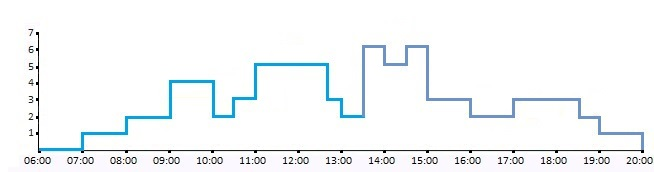
\includegraphics[width=1.0\textwidth]{reqshiftbreak1}
  \caption{The needed workers over planning period is shown with the blue line.}
  \label{fig:reqshiftbreak1} 
\end{figure}

\item  $shiftMinusRequirement_t : $ There are several shifts, that are characterized with start $s_i.start$ and length $s_i.length$ of shift $s_i$. First, we need to convert each shift $s_i$ with a number of workers $s_i.w_j$ in  each day $j$ to the number of people working in each time slot $t$. We need to calculate this working staff decreased by requirements of workers $shiftMinusRequirement_t$ in each time slot $t$ . In this calculation, we are not considering the breaks of workers. In Figure~\ref{fig:reqshiftbreak2} is shown an example graph with required employees and present employees (shifts without breaks). The breaks will fill these space between two curves, as it is shown in Figure~\ref{fig:reqshiftbreak3}.

\begin{equation}
shiftMinusRequirement_t \ge 0 \quad \forall t = 1, 2, ..., n
\end{equation}


\begin{figure}[h]
  \centering
  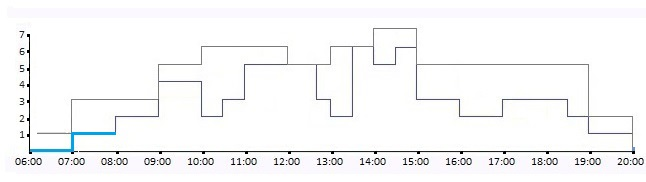
\includegraphics[width=1.0\textwidth]{reqshiftbreak2}
  \caption{Shifts are scheduled without breaks, The required workers (Blue Line) and present workers (Gray Line) are shown over planning period.}
  \label{fig:reqshiftbreak2} 
\end{figure}

\begin{figure}[h]
  \centering
  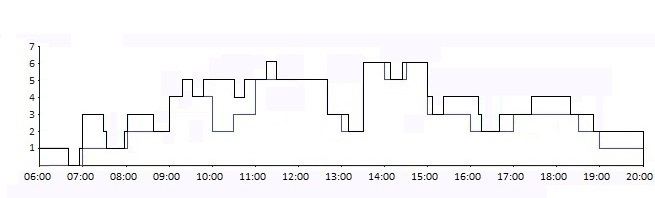
\includegraphics[width=1.0\textwidth]{reqshiftbreak3}
  \caption{ Breaks are assigned to each shift, The required employees (Blue Line) and working employees (Black Line) are shown over planning period.}
  \label{fig:reqshiftbreak3} 
\end{figure}


To calculate the number of workers in each time slot between these two curves, we use Algorithm~\ref{alg:convert-shifts}, is given above,

\begin{algorithm}
  \SetKw{BreakFor}{break for}
  \KwIn{$r_t$, $s_i.start$, $s_i.length$, $s_i.w_j$ }
  \KwOut{$shiftMinusRequirement_t$}
  \For{$t\leftarrow 0$ \KwTo n-1}
  {
    $shiftMinusRequirement_t = -  r_t$
  }
  \For{$i\leftarrow 0$ \KwTo Number of Shifts -1}
  {
     \For{$j\leftarrow 0$ \KwTo 6}
     {
        \For{$l\leftarrow 0$ \KwTo $s_i.length -1$}
        {
		 $shiftMinusRequirement[(s_i.start + l + n * j/7) \%n] += s_i.w_j$  ;
        }
     }
  }
  \Return{$shiftMinusRequirement_t$;}
  \caption{Convert Shift Schedules to the number of Assigned Workers in Each Time Slot}
  \label{alg:convert-shifts} 
\end{algorithm}


In the Algorithm~\ref{alg:convert-shifts}, first we set the $shiftMinusRequirement_t$ variable with the minus needed number of workers in each time slot $t$ (Line $2$).  The number of day cycle is considered $7$ days (a week) for break scheduling problem (Line $5$). Each day has $n/7$ time slots. Suppose that the $slotlength$ is equal to 5, time slots [0- 288) is the interval of the first day, second day is between [288, 576), .. , [1928, 0) is the interval of last day. 

The night shifts of last day continue to the beginning of the week, due to the cyclic structure. Therefore, we need to apply $\mod n$. In line $7$, the day number is converted to the first time slot of a day with $(n * j / 7) (\mod n)$ and we add the equation $s_i.start + l$  to calculate the each time slot $t$ belongs to the interval of shift $s_i$ on day $j$. The right side of the equation is equal to the number of employees in day $j$ and shift $s_i$. \\

\item As mentioned in \cite{li:2010:beer}, the common settings and the initialization of the used parameters in our formulation for the soft constraints $C0$ to $C6$ are given below (The weight constraints of soft constraints are initialised with $W_i \quad \forall i = \{ 0, 1, 2...6 \}$. ),

\begin{itemize}
\item $C_0 : $ The earliest start of the break $earliestStart$ is half an hour after the beginning of the shift and the latest end $latestEnd$ half an hour before the shift's end. The exception of this soft constraint is evaluated with the weight $W_0$ is 20. \\

\item $C_1 : $ The earliest start of the lunch break $lunchEarliestStart$ is $03:30$ hours and the latest end $lunchLatestEnd$ $06:00$ hours after the beginning of the shift. The weight value  $W_1$ of this constraint is equal to $10$. \\

\item $C_2 : $ Work periods are the durations of work between the breaks and also between the first break and start of a shift and the last break and end of a shift. These durations need to be between two parameters, that are the minimum length of work period $minWP$ and maximum length of work period $maxWP$. These parameters are set $00.30$ and $01:40$ and the weight value $W_2$ is equal to 20.  

Meanwhile, if the start time of the first break is before the earliest start and the end time of the last break is after the latest end, this situation violates two soft constraints, that are $C_0$ and $C_2$. \\

\item $C_3 : $ Employees need to have more break time $minBreakExceedsWorkLimit$, if they exceed a certain limit $workLimit$. This constraint is violated, after 50 minutes of the work period, have less than 20 minutes break and the weight value $W_3$ is equal to $20$.  \\

\item $C_4 : $ The break duration of employees needs not to be  less than 10 minutes ($minBreakLength$) and not more than one hour ($maxBreakLength$). The less and more break duration is evaluated with the weight, $W_4$ is 1. \\

\item $C_5 : $ Sum of the shortages of employees in each time interval during the planning period. The weight value  $W_5$ for each shortage is equal to $10$. \\

\item $C_6 : $ Sum of the excesses of employees in each time interval during the planning period. The weight value  $W_6$  for each excess is equal to $ 2$ .
\end{itemize}

Beer et. al in \cite{li:2010:beer} mentioned that in real world benchmarks, most of these constraints violations ($C_0$, $C_1$, $C_2$, $C_3$, $C_4$) are less than 5 percent for each instance, with respect to the weight values above. Therefore, we initialize our variables based on satisfying these first five constraints and evaluate the objective function with the remaining two soft constraints, that are excesses and shortages of workers in each time interval during the planning period. \\


\end{itemize}



\subsubsection{Decision Variables}

The proposed integer linear programming formulation for break scheduling problem, the decision variables are given below,

\subsubsection{Initialization of Breaks}

Each shift-day-duty $s$ have several breaks. We initialize these breaks with three types of break variables, based on different time windows $TW_i$ ($i = \{0,1,2 \}$ is the number of break type ). These three break types are $bl_{sbt}$, $l_{sbt}$, $al_{sbt}$.



In break scheduling problem, breaks can be assigned into time slot $t$ between the earliest start of the break $earliestStart$ and the latest end of the break $latestEnd$. Thus, $C_0$ constraint needs to be satisfied and the breaks must be into these intervals. These three break type variables are assigned true, if there exists a start of a break in the time slot $t$. 

\begin{equation}
bl_{sbt} = \left\{ \begin{array}{cc}
		1 & \mbox{if shift-day-duty $s$ have break $b$ before lunch, starts from time slot $t$} \\
		0 & \mbox{otherwise}
	    \end{array}
    \right.
\end{equation}

\begin{equation}
l_{st} = \left\{ \begin{array}{cc}
		1 & \mbox{if shift-day-duty $s$ have lunch break, starts from time slot $t$} \\
		0 & \mbox{otherwise}
	    \end{array}
    \right.
\end{equation}


\begin{equation}
al_{sbt} = \left\{ \begin{array}{cc}
		1 & \mbox{if shift-day-duty $s$ have break $b$ after lunch, starts from time slot $t$} \\
		0 & \mbox{otherwise}
	    \end{array}
    \right.
\end{equation}


These time slots are restricted with different time windows, based on types of breaks.  We are assuming that every staff has three monitor breaks before the lunch break and $m-4$ monitor breaks after the lunch break depends on $s_i.breakTime$ of shift $s_i$. We will present them as follows, and explain time windows in details:
\begin{itemize}

\item $bl_{sbt}$ : We assumed each shift-day-duty $s$ have three monitor breaks before lunch. We need to consider the followings to reduce the time window $TW_0$ (earliest and latest possible start) of this type of breaks, 


\begin{itemize}
\item[-] The earliest start of the before lunch breaks, based on constraint $C_0$, at  earliest start of the break $earliestStart$.
\item[-] These breaks are before the lunch break, therefore the latest start of a before lunch breaks can be the latest end of lunch break of a shift, based on constraint $C_1$. As an example with shift length 8 hours, the time window of before lunch break (Red) is illustrated below, \\

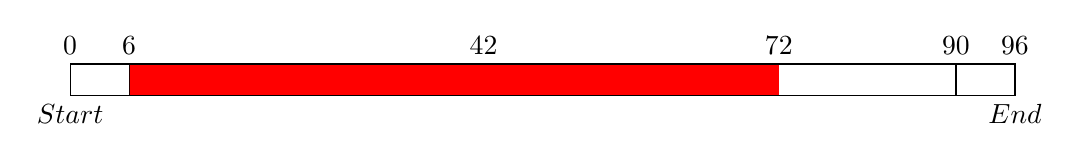
\begin{tikzpicture}

%draw horizontal line
\draw (0,0.2) rectangle (12,-0.2);

%draw vertical lines
\foreach \x in {0,0.75,9,11.25,12}
\draw (\x cm,5.5pt) -- (\x cm,-5.5pt);



\draw (0,0) node[above=5.5pt] {$ 0 $} node[below=5.5pt] {$ Start  $};
\draw (0.75,0) node[above=5.5pt] {$ 6 $};

\draw (5.25,0) node[above=5.5pt] {$ 42 $};
\draw (9,0) node[above=5.5pt] {$ 72 $};

\draw (11.25,0) node[above=5.5pt] {$ 90 $};
\draw (12,0) node[above=5.5pt] {$ 96 $} node[below=5.5pt] {$ End $};

\draw[line width=11pt, color=red] (0.76,0) rectangle (9, 0)[above=3pt];
\end{tikzpicture}


\item[-] We can still restrict the time window $TW_0$. We need to consider that employees have a lunch break after these breaks and before the latest end of lunch break. The employees can have their lunch break as latest in the end of the lunch break period (last 6 time slots) and before the lunch break, the staff must work minimum 6 time slots ($minWP$), due to the constraint $C_2$. 

\item[-] The monitor break variables have length of 2 time slots. Consider time slot $t$ is the start time of the break, we need to decrease 2 more time slots from the latest start of the before lunch breaks. The illustrated example of the restricted time window of before lunch break with shift length 8 is shown below (Red: Time Window of Before Lunch Break, Black: Monitor Break, Yellow: Minimum Working Period, Blue: Lunch Break), \\

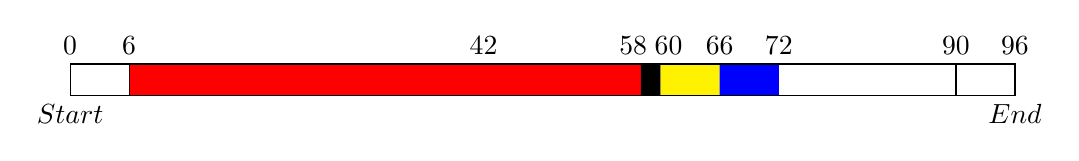
\begin{tikzpicture}

%draw horizontal line
\draw (0,0.2) rectangle (12,-0.2);

%draw vertical lines
\foreach \x in {0,0.75,9,11.25,12}
\draw (\x cm,5.5pt) -- (\x cm,-5.5pt);



\draw (0,0) node[above=5.5pt] {$ 0 $} node[below=5.5pt] {$ Start  $};
\draw (0.75,0) node[above=5.5pt] {$ 6 $};

\draw (5.25,0) node[above=5.5pt] {$ 42 $};
\draw (7.15,0) node[above=5.5pt] {$ 58 $};
\draw (7.6,0) node[above=5.5pt] {$ 60 $};
\draw (8.25,0) node[above=5.5pt] {$ 66 $};
\draw (9,0) node[above=5.5pt] {$ 72 $};

\draw (11.25,0) node[above=5.5pt] {$ 90 $};
\draw (12,0) node[above=5.5pt] {$ 96 $} node[below=5.5pt] {$ End $};

\draw[line width=11pt, color=red] (0.76,0) rectangle (7.25, 0)[above=3pt];
\draw[line width=11pt, color=black] (7.25,0) rectangle (7.5, 0)[above=3pt];
\draw[line width=11pt, color=yellow] (7.5,0) rectangle (8.25, 0)[above=3pt];
\draw[line width=11pt, color=blue] (8.25,0) rectangle (9, 0)[above=3pt];

\end{tikzpicture}
\end{itemize}

From the restrictions above, the time window of before lunch breaks is calculated below,

\begin{equation}
es_0  = earliestStart
\end{equation}

\begin{equation}
ls_0 = lunchLatestEnd - lunchBreakTime- minWP -2
\end{equation}

The time windows of these three breaks are also tightened between each other from the following statements,

\begin{itemize}
\item[-]  The earliest start of the first before lunch break is the earliest start of the break $earliestStart$. However, it must end before the other remaining two before lunch breaks. Therefore, we consider the last before lunch break starts at the latest start of the time window above. Before this break the employee need to work $minWP$. The second break finishes at latest at this point of time. Therefore, if we decrease 2 time slots (length of second break) and $minWP$ (between the first and second break), we can find the latest point of the end of the first break. At last, we need to decrease 2 more time slot to find the latest start of the first before lunch break. The illustrated example  of the restricted time window for the first before lunch break is given below (Red : Time Window of Before Lunch Break, Black: Monitor Break, Yellow: Minimum Working Period, Blue: Lunch Break), \\


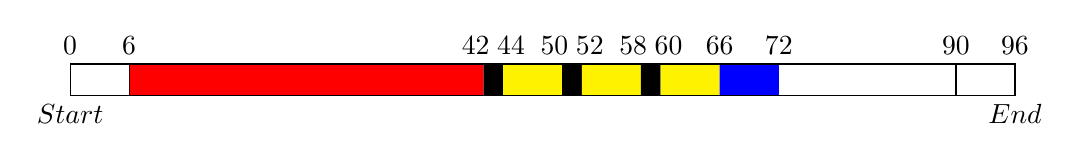
\begin{tikzpicture}
%draw horizontal line
\draw (0,0.2) rectangle (12,-0.2);

%draw vertical lines
\foreach \x in {0,0.75,9,11.25,12}
\draw (\x cm,5.5pt) -- (\x cm,-5.5pt);

\draw (0,0) node[above=5.5pt] {$ 0 $} node[below=5.5pt] {$ Start  $};
\draw (0.75,0) node[above=5.5pt] {$ 6 $};

\draw (5.15,0) node[above=5.5pt] {$ 42 $};
\draw (5.6,0) node[above=5.5pt] {$ 44 $};
\draw (6.15,0) node[above=5.5pt] {$ 50 $};
\draw (6.6,0) node[above=5.5pt] {$ 52 $};
\draw (7.15,0) node[above=5.5pt] {$ 58 $};
\draw (7.6,0) node[above=5.5pt] {$ 60 $};
\draw (8.25,0) node[above=5.5pt] {$ 66 $};
\draw (9,0) node[above=5.5pt] {$ 72 $};

\draw (11.25,0) node[above=5.5pt] {$ 90 $};
\draw (12,0) node[above=5.5pt] {$ 96 $} node[below=5.5pt] {$ End $};

\draw[line width=11pt, color=red] (0.76,0) rectangle (5.25, 0)[above=3pt];
\draw[line width=11pt, color=black] (5.25,0) rectangle (5.5, 0)[above=3pt];
\draw[line width=11pt, color=yellow] (5.5,0) rectangle (6.25, 0)[above=3pt];
\draw[line width=11pt, color=black] (6.25,0) rectangle (6.5, 0)[above=3pt];
\draw[line width=11pt, color=yellow] (6.5,0) rectangle (7.25, 0)[above=3pt];
\draw[line width=11pt, color=black] (7.25,0) rectangle (7.5, 0)[above=3pt];
\draw[line width=11pt, color=yellow] (7.5,0) rectangle (8.25, 0)[above=3pt];
\draw[line width=11pt, color=blue] (8.25,0) rectangle (9, 0)[above=3pt];


\end{tikzpicture}
\item[-] We have already calculated the latest start of the second break, that is $minWP + 2$ time slots before the old latest start. The earliest start of the second before lunch break must be after the first break, therefore, we need to add to the first before lunch break, $minWP + 2$ time slots, to the earliest start of the break. As an example of the restricted time window for the second before lunch break is shown below (Red : Time Window of Before Lunch Break, Black : Monitor Break, Yellow : Minimum Working Period, Blue : Lunch Break), \\


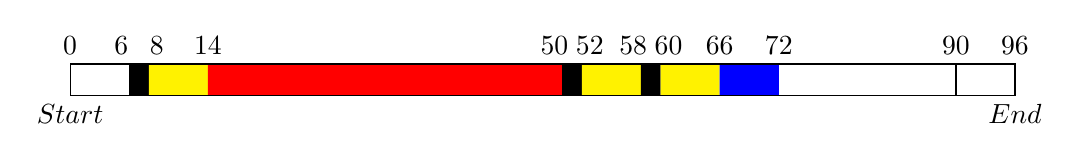
\begin{tikzpicture}
%draw horizontal line
\draw (0,0.2) rectangle (12,-0.2);

%draw vertical lines
\foreach \x in {0,0.75,9,11.25,12}
\draw (\x cm,5.5pt) -- (\x cm,-5.5pt);



\draw (0,0) node[above=5.5pt] {$ 0 $} node[below=5.5pt] {$ Start  $};
\draw (0.65,0) node[above=5.5pt] {$ 6 $};
\draw (1.1,0) node[above=5.5pt] {$ 8 $};
\draw (1.75,0) node[above=5.5pt] {$ 14 $};
\draw (6.15,0) node[above=5.5pt] {$ 50 $};
\draw (6.6,0) node[above=5.5pt] {$ 52 $};
\draw (7.15,0) node[above=5.5pt] {$ 58 $};
\draw (7.6,0) node[above=5.5pt] {$ 60 $};
\draw (8.25,0) node[above=5.5pt] {$ 66 $};
\draw (9,0) node[above=5.5pt] {$ 72 $};

\draw (11.25,0) node[above=5.5pt] {$ 90 $};
\draw (12,0) node[above=5.5pt] {$ 96 $} node[below=5.5pt] {$ End $};

\draw[line width=11pt, color=black] (0.76,0) rectangle (1.0, 0)[above=3pt];
\draw[line width=11pt, color=yellow] (1.0,0) rectangle (1.75, 0)[above=3pt];
\draw[line width=11pt, color=red] (1.75,0) rectangle (6.25, 0)[above=3pt];
\draw[line width=11pt, color=black] (6.25,0) rectangle (6.5, 0)[above=3pt];
\draw[line width=11pt, color=yellow] (6.5,0) rectangle (7.25, 0)[above=3pt];
\draw[line width=11pt, color=black] (7.25,0) rectangle (7.5, 0)[above=3pt];
\draw[line width=11pt, color=yellow] (7.5,0) rectangle (8.25, 0)[above=3pt];
\draw[line width=11pt, color=blue] (8.25,0) rectangle (9, 0)[above=3pt];


\end{tikzpicture}
\item[-] With the same rule, the third before lunch break must start after $2 *  (minWP + 2)$ from earliest start of the break and latest start is the old latest start, that we calculated above. The illustrated example  of the restricted time window for the last before lunch break is given below (Red : Time Window of Before Lunch Break, Black : Monitor Break, Yellow : Minimum Working Period, Blue : Lunch Break), \\


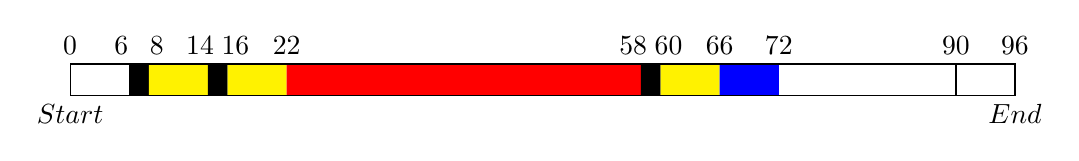
\begin{tikzpicture}

%draw horizontal line
\draw (0,0.2) rectangle (12,-0.2);

%draw vertical lines
\foreach \x in {0,0.75,9,11.25,12}
\draw (\x cm,5.5pt) -- (\x cm,-5.5pt);



\draw (0,0) node[above=5.5pt] {$ 0 $} node[below=5.5pt] {$ Start  $};
\draw (0.65,0) node[above=5.5pt] {$ 6 $};
\draw (1.1,0) node[above=5.5pt] {$ 8 $};
\draw (1.65,0) node[above=5.5pt] {$ 14 $};
\draw (2.1,0) node[above=5.5pt] {$ 16 $};
\draw (2.75,0) node[above=5.5pt] {$ 22 $};
\draw (7.15,0) node[above=5.5pt] {$ 58 $};
\draw (7.6,0) node[above=5.5pt] {$ 60 $};
\draw (8.25,0) node[above=5.5pt] {$ 66 $};
\draw (9,0) node[above=5.5pt] {$ 72 $};

\draw (11.25,0) node[above=5.5pt] {$ 90 $};
\draw (12,0) node[above=5.5pt] {$ 96 $} node[below=5.5pt] {$ End $};

\draw[line width=11pt, color=black] (0.76,0) rectangle (1.0, 0)[above=3pt];
\draw[line width=11pt, color=yellow] (1.0,0) rectangle (1.75, 0)[above=3pt];
\draw[line width=11pt, color=black] (1.75,0) rectangle (2.0, 0)[above=3pt];
\draw[line width=11pt, color=yellow] (2.0,0) rectangle (2.75, 0)[above=3pt];
\draw[line width=11pt, color=red] (2.75,0) rectangle (7.25, 0)[above=3pt];
\draw[line width=11pt, color=black] (7.25,0) rectangle (7.5, 0)[above=3pt];
\draw[line width=11pt, color=yellow] (7.5,0) rectangle (8.25, 0)[above=3pt];
\draw[line width=11pt, color=blue] (8.25,0) rectangle (9, 0)[above=3pt];

\end{tikzpicture}
\end{itemize}


As a summary, we added $i * ( minWP +2 )$ to the earliest start of a break and decrease $(2 - i) * ( minWP +2 )$ from the latest start where $i$ indicating the number of before lunch break -1. The updated interval of time window $TW_0$ of before lunch break is given below,

\begin{equation}
es_0  = earliestStart + i * ( minWP +2 ) 
\end{equation}

\begin{equation}
ls_0 = lunchLatestEnd - lunchBreakTime-  (3 - i) * ( minWP + 2 ) 
\end{equation}
\begin{equation}
 \forall i = \{0,1,2\}
\end{equation}


\item $l_{st}$ : The shifts have at most one lunch break, therefore this variable is initialized with two dimensions shift-day-duty $s$ and time slot $t$. The lunch break can be between the Lunch Earliest Start and Lunch Latest End - Lunch Break Time. This break has length 6 time slots. The illustration of time window $TW_1$  of lunch break is shown below, (Blue: Time Window of Lunch Break, Black: Lunch Break), \\

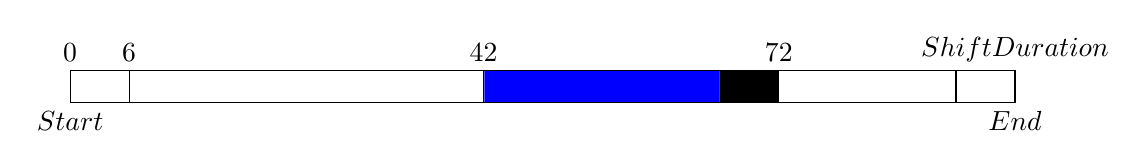
\begin{tikzpicture}

%draw horizontal line
\draw (0,0.2) rectangle (12,-0.2);

%draw vertical lines
\foreach \x in {0,0.75,5.25,9,11.25,12}
\draw (\x cm,5.5pt) -- (\x cm,-5.5pt);

\draw (0,0) node[above=5.5pt] {$ 0 $} node[below=5.5pt] {$ Start  $};
\draw (0.75,0) node[above=5.5pt] {$ 6 $};

\draw (5.25,0) node[above=5.5pt] {$ 42 $};
\draw (9,0) node[above=5.5pt] {$ 72 $};


\draw (12,0) node[above=5.5pt] {$ Shift Duration $} node[below=5.5pt] {$ End $};


\draw[line width=11pt, color=blue] (5.26, 0) rectangle (8.25, 0)[above=3pt];
\draw[line width=11pt, color=black] (8.25,0) rectangle (9, 0)[above=3pt];
\end{tikzpicture}

The earliest start and latest start of a lunch break is given below,

\begin{equation}
es_1 =  Lunch Earliest Start 
\end{equation}

\begin{equation}
ls_1 =  Lunch Latest End - Lunch Break Time
\end{equation}

\item $al_{sbt}$ : We assumed each shift-day-duty $s$ have $m-4$ monitor breaks after lunch, based on length of the shift. We need to consider the followings to calculate the time window $TW_2$ of these types of breaks, 

\begin{itemize}

\item[-] The latest start of the after lunch breaks, based on constraint $C_0$, at  latest end of the break $latestEnd$. 

\item[-] These breaks are after the lunch break, therefore the earliest start can be the  earliest start of lunch break of a shift. As an example with shift length 8 hours, the time window of after lunch break (Green) is illustrated below, \\

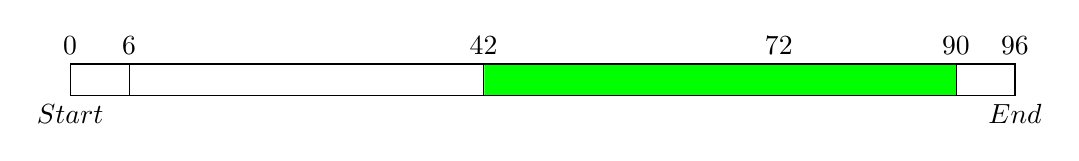
\begin{tikzpicture}

%draw horizontal line
\draw (0,0.2) rectangle (12,-0.2);

%draw vertical lines
\foreach \x in {0,0.75,5.25,9,11.25,12}
\draw (\x cm,5.5pt) -- (\x cm,-5.5pt);

\draw (0,0) node[above=5.5pt] {$ 0 $} node[below=5.5pt] {$ Start  $};
\draw (0.75,0) node[above=5.5pt] {$ 6 $};

\draw (5.25,0) node[above=5.5pt] {$ 42 $};
\draw (9,0) node[above=5.5pt] {$ 72 $};

\draw (11.25,0) node[above=5.5pt] {$ 90 $};
\draw (12,0) node[above=5.5pt] {$ 96 $} node[below=5.5pt] {$ End $};

\draw[line width=11pt, color=green] (5.26, 0) rectangle (11.25, 0)[above=3pt];
\end{tikzpicture}


\item[-] Likewise, in before lunch break, we can also reduce the time window $TW_2$ of after lunch break. We need to consider that employees have a lunch break before these breaks. Therefore, assuming the employees have lunch break in the beginning of the lunch break period (first 6 time slot) and after the lunch, the staff must have a working period minimum 6 time slots, due to the constraint $C_2$. 

\item[-]  The monitor break variables have a length of 2 time slots. Consider time slot $t$ is the start time of the break, we need to decrease 2 time slot from the latest end of the break  $latestEnd$. The illustrated example of the restricted time window of after lunch break with shift length 8 is shown below (Green : Time Window of After Lunch Break, Black : Monitor Break, Yellow : Minimum Working Period, Blue : Lunch Break), \\


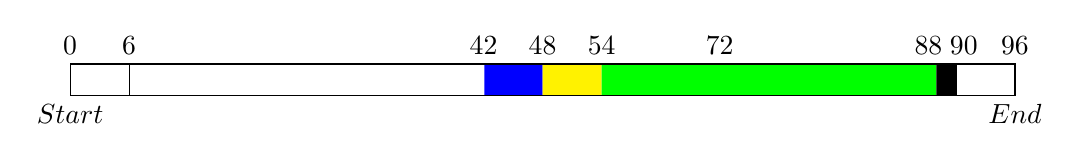
\begin{tikzpicture}

%draw horizontal line
\draw (0,0.2) rectangle (12,-0.2);

%draw vertical lines
\foreach \x in {0,0.75,9,11.25,12}
\draw (\x cm,5.5pt) -- (\x cm,-5.5pt);



\draw (0,0) node[above=5.5pt] {$ 0 $} node[below=5.5pt] {$ Start  $};
\draw (0.75,0) node[above=5.5pt] {$ 6 $};

\draw (5.25,0) node[above=5.5pt] {$ 42 $};
\draw (6,0) node[above=5.5pt] {$ 48 $};
\draw (6.75,0) node[above=5.5pt] {$ 54 $};
\draw (8.25,0) node[above=5.5pt] {$ 72 $};
\draw (10.9,0) node[above=5.5pt] {$ 88 $};

\draw (11.35,0) node[above=5.5pt] {$ 90 $};
\draw (12,0) node[above=5.5pt] {$ 96 $} node[below=5.5pt] {$ End $};

\draw[line width=11pt, color=blue] (5.26,0) rectangle (6, 0)[above=3pt];
\draw[line width=11pt, color=yellow] (6,0) rectangle (6.75, 0)[above=3pt];
\draw[line width=11pt, color=green] (6.75, 0) rectangle (11.00, 0)[above=3pt];
\draw[line width=11pt, color=black] (11.00, 0) rectangle (11.25, 0)[above=3pt];
\end{tikzpicture}
\end{itemize}

As we explained in before lunch breaks, we can also restrict the time window of each after lunch break $TW_2$ between each other. We add i * ( minWP +2 ) to earliest start of after lunch break and decrease  (m - 5- i) * ( minWP +2 ) from latest start of after lunch break where $i$ indicating the number of after lunch break -1. From the all restrictions above, the earliest and latest start of after lunch breaks are calculated as given below,

\begin{equation}
es_2 = Lunch Earliest Start + Lunch Break Time + minWP * ( i +1) +2 i  
\end{equation}

\begin{equation}
ls_2 = Latest End - 2 - (m - 5 -  i) *  (2 +  minWP)  
\end{equation}

\begin{equation}
\forall i = \{0,1, .. , m-5\}
\end{equation}


The illustrated example of the restricted time window for the first after lunch break with shift length 8 is given below (Green: Time Window of After Lunch Break, Black: Monitor Break, Yellow: Minimum Working Period, Blue: Lunch Break), \\

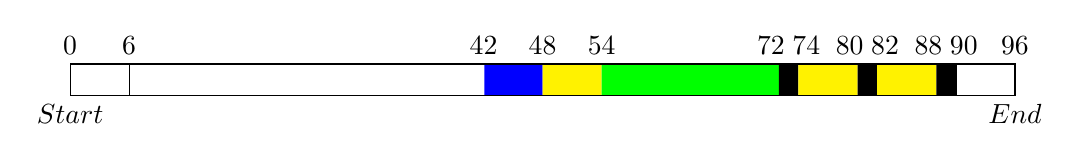
\begin{tikzpicture}
%draw horizontal line
\draw (0,0.2) rectangle (12,-0.2);

%draw vertical lines
\foreach \x in {0,0.75,9,11.25,12}
\draw (\x cm,5.5pt) -- (\x cm,-5.5pt);

\draw (0,0) node[above=5.5pt] {$ 0 $} node[below=5.5pt] {$ Start  $};
\draw (0.75,0) node[above=5.5pt] {$ 6 $};

\draw (5.25,0) node[above=5.5pt] {$ 42 $};
\draw (6,0) node[above=5.5pt] {$ 48 $};
\draw (6.75,0) node[above=5.5pt] {$ 54 $};
\draw (8.9,0) node[above=5.5pt] {$ 72 $};
\draw (9.35,0) node[above=5.5pt] {$ 74 $};
\draw (9.9,0) node[above=5.5pt] {$80 $};
\draw (10.35,0) node[above=5.5pt] {$ 82 $};
\draw (10.9,0) node[above=5.5pt] {$ 88 $};
\draw (11.35,0) node[above=5.5pt] {$ 90 $};
\draw (12,0) node[above=5.5pt] {$ 96 $} node[below=5.5pt] {$ End $};


\draw[line width=11pt, color=blue] (5.26,0) rectangle (6, 0)[above=3pt];
\draw[line width=11pt, color=yellow] (6,0) rectangle (6.75, 0)[above=3pt];
\draw[line width=11pt, color=green] (6.75, 0) rectangle (9.00, 0)[above=3pt];
\draw[line width=11pt, color=black] (9,0) rectangle (9.25, 0)[above=3pt];
\draw[line width=11pt, color=yellow] (9.25,0) rectangle (10, 0)[above=3pt];
\draw[line width=11pt, color=black] (10,0) rectangle (10.25, 0)[above=3pt];
\draw[line width=11pt, color=yellow] (10.25,0) rectangle (11, 0)[above=3pt];
\draw[line width=11pt, color=black] (11.00, 0) rectangle (11.25, 0)[above=3pt];

\end{tikzpicture}

The second after lunch break  with shift length 8 is shown below (Green: Time Window of After Lunch Break, Black: Monitor Break, Yellow: Minimum Working Period, Blue: Lunch Break), \\


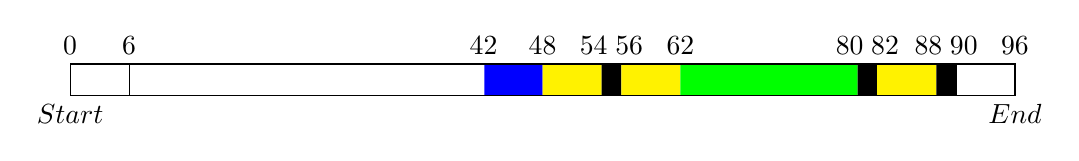
\begin{tikzpicture}
%draw horizontal line
\draw (0,0.2) rectangle (12,-0.2);

%draw vertical lines
\foreach \x in {0,0.75,9,11.25,12}
\draw (\x cm,5.5pt) -- (\x cm,-5.5pt);




\draw (0,0) node[above=5.5pt] {$ 0 $} node[below=5.5pt] {$ Start  $};
\draw (0.75,0) node[above=5.5pt] {$ 6 $};

\draw (5.25,0) node[above=5.5pt] {$ 42 $};
\draw (6,0) node[above=5.5pt] {$ 48 $};
\draw (6.65,0) node[above=5.5pt] {$ 54 $};
\draw (7.1,0) node[above=5.5pt] {$ 56 $};
\draw (7.75,0) node[above=5.5pt] {$ 62 $};
\draw (9.9,0) node[above=5.5pt] {$80 $};
\draw (10.35,0) node[above=5.5pt] {$ 82 $};
\draw (10.9,0) node[above=5.5pt] {$ 88 $};
\draw (11.35,0) node[above=5.5pt] {$ 90 $};
\draw (12,0) node[above=5.5pt] {$ 96 $} node[below=5.5pt] {$ End $};

\draw[line width=11pt, color=blue] (5.26,0) rectangle (6, 0)[above=3pt];
\draw[line width=11pt, color=yellow] (6,0) rectangle (6.75, 0)[above=3pt];
\draw[line width=11pt, color=black] (6.75,0) rectangle (7, 0)[above=3pt];
\draw[line width=11pt, color=yellow] (7,0) rectangle (7.75, 0)[above=3pt];
\draw[line width=11pt, color=green] (7.75, 0) rectangle (10.00, 0)[above=3pt];
\draw[line width=11pt, color=black] (10,0) rectangle (10.25, 0)[above=3pt];
\draw[line width=11pt, color=yellow] (10.25,0) rectangle (11, 0)[above=3pt];
\draw[line width=11pt, color=black] (11.00, 0) rectangle (11.25, 0)[above=3pt];


\end{tikzpicture}

The illustrated example  of the restricted time window for the last after lunch break  with shift length 8 is given below (Green: Time Window of After Lunch Break, Black: Monitor Break, Yellow: Minimum Working Period, Blue: Lunch Break), \\


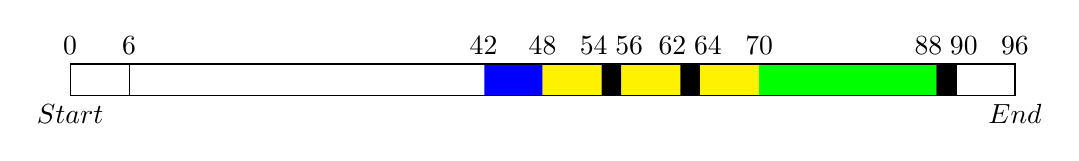
\begin{tikzpicture}

%draw horizontal line
\draw (0,0.2) rectangle (12,-0.2);

%draw vertical lines
\foreach \x in {0,0.75,9,11.25,12}
\draw (\x cm,5.5pt) -- (\x cm,-5.5pt);

\draw (0,0) node[above=5.5pt] {$ 0 $} node[below=5.5pt] {$ Start  $};
\draw (0.75,0) node[above=5.5pt] {$ 6 $};

\draw (5.25,0) node[above=5.5pt] {$ 42 $};
\draw (6,0) node[above=5.5pt] {$ 48 $};
\draw (6.65,0) node[above=5.5pt] {$ 54 $};
\draw (7.1,0) node[above=5.5pt] {$ 56 $};
\draw (7.65,0) node[above=5.5pt] {$ 62 $};
\draw (8.1,0) node[above=5.5pt] {$64 $};
\draw (8.75,0) node[above=5.5pt] {$ 70 $};
\draw (10.9,0) node[above=5.5pt] {$ 88 $};
\draw (11.35,0) node[above=5.5pt] {$ 90 $};
\draw (12,0) node[above=5.5pt] {$ 96 $} node[below=5.5pt] {$ End $};

\draw[line width=11pt, color=blue] (5.26,0) rectangle (6, 0)[above=3pt];
\draw[line width=11pt, color=yellow] (6,0) rectangle (6.75, 0)[above=3pt];
\draw[line width=11pt, color=black] (6.75,0) rectangle (7, 0)[above=3pt];
\draw[line width=11pt, color=yellow] (7,0) rectangle (7.75, 0)[above=3pt];
\draw[line width=11pt, color=black] (7.75,0) rectangle (8, 0)[above=3pt];
\draw[line width=11pt, color=yellow] (8,0) rectangle (8.75, 0)[above=3pt];
\draw[line width=11pt, color=green] (8.75, 0) rectangle (11.00, 0)[above=3pt];
\draw[line width=11pt, color=black] (11.00, 0) rectangle (11.25, 0)[above=3pt];

\end{tikzpicture}








\end{itemize}























\begin{itemize}

\item $st_{sb}$ : Start time is an integer positive variable, indicating the time slot of the start of the breaks within their shift. Every break $b$ of shift-day-duty $s$ have a start time and the value of start time is between this interval below, 


\begin{equation}
 0 \le st_{sb} \le  Shift Length -Earliest Start -Latest End - 2  
\end{equation} 
\begin{equation}
\forall s = \{0, 1 ...sdd -1\} \quad \forall b = \{0, 1, ...,m -1 \}
\end{equation} 

We needed the start time of each break to calculate work period between each other. The equation to calculate the start time will be explained in constraint section.




\item $wp_{sb}$ : There are two soft constraints based on a work period in the problem statement, however, as we mentioned before, we added this constraint directly to our initialization of the problem. $wp_{sb}$ is defined as follows,

\begin{itemize}
\item  The duration from the start time of the shift to the beginning of first break.
\item  The duration from the end time of  each break to the start time of the following break belongs to the same shift-day-duty.
\item  The duration from the end of the last break to the end of the shift.
\end{itemize}

We initialize the work period $wp_{sb}$  variable, based on start time $st_{sb}$ in the constraint section more clearly. This variable must be due to constraint $C_2$ between the interval [00:30, 01:40].

Based on the constraint $C_3$, if an employee exceeds 50 minute work period, he must have 20 minutes break. Each monitor break has 10 minutes length. Therefore, we initialize each work period have between 30 minutes to 50 minutes long, except two working periods. These two working periods are,

\begin{itemize}
\item The working period before the lunch break, because the lunch break is 30 minutes long, therefore the employee can exceed 50 minutes working period before. \\
\item The working period after the last break. Because, the employee will finish his duty and will be free.
\end{itemize}


We initialize the each working period between interval, 

\begin{equation}
00:30 \le wp_{sb} \le 01:40 \quad \forall s = \{0, 1 ...sdd -1\} \quad \forall b = \{0, 1, ..., m\}
\end{equation} 

We add the constraint whether working period is less or equal to 50 minutes or not in the following section. 

\item We added first five soft constraints into our formulation as an hard constraint. The remaining two components of the objective function are :
\begin{itemize}
\item $C_5$ : Sum of excesses of employees in each time slot. 

\item $C_6$ : Sum of shortages of employees in each time slot. \\
\end{itemize} 

\item To calculate these two components, we needed two variables $ex_t$, $sh_t$ like in shift design problem, 
\begin{itemize}
\item $ex_t$ : Excesses  of workers in time slot $t$.

\item $sh_t$ : Shortages of workers in time slot $t$. \\
\end{itemize}
\end{itemize}

\subsection{Constraints}
We will present the constraints, we use in our integer programming formulation in 2 sections, soft and hard constraints. 


\subsubsection{Hard Constraints}

\begin{itemize}
\item Each break of shift-day-duty $s$ must assign to exactly one time slot $t$. For each break type the equations are shown below,

\begin{itemize}
\item For before lunch breaks $bl_{sbt}$,


\begin{equation}
\sum_{t \in TW_0 } bl_{sbt} = 1 \quad \forall s = \{0, 1, ..., sdd -1\} \quad  \forall b = \{0, 1, 2\}
\end{equation}

\item For lunch breaks $l_{st}$,

\begin{equation}
\sum_{t \in TW_1} l_{st} = 1 \quad \forall s = \{0, 1, ...,sdd -1\} 
\end{equation}

\item For after lunch breaks $al_{sbt}$,

\begin{equation}
\sum_{t \in TW_2} al_{sbt} = 1 \quad  \forall s = \{0, 1, ...,sdd -1\} \quad \forall b = \{0, 1, ...,m - 4\}
\end{equation}


\end{itemize} 



\item $st_{sb} : $ Start time variable indicates the time difference between the break $b$ start and the belonging shift start $s_i.start$. The start times of each break are initialized based on each break type, are given below,


\begin{itemize}
\item  The dimension $t$ in variable $bl_{sbt}$, represent the start point of a break after the earliest start of before lunch breaks. We calculate the earliest start of the before lunch breaks $es_0$ as Earliest Start +$ (minWP + 2) * i$, where $i$ is indicating the number of before lunch break. $st_{sb}$ is initialized for each before lunch break as follows,

\begin{equation}
st_{sb} =es_0 + t * bl_{sbt} \quad \forall s = \{0, 1 ...sdd -1\} \quad \forall t \in TW_0 \quad \forall b = \{0, 1, 2\}
\end{equation}

\item There is just one lunch break and it is the fourth break (b = 3). The earliest start of the lunch break $es_1$ is lunch earliest start. The initialization of it, is given below,

\begin{equation}
st_{s3} =  es_1 + t * l_{st} \quad \forall s = \{0, 1 ...sdd -1\} \quad \forall t \in TW_1
\end{equation}

\item The earliest start of the after lunch breaks  $es_2$ is  initialized as Lunch Earliest Start + Lunch Break Time + $minWP + (minWP + 2) * i$ where $i$ is representing the number of after lunch break. The start times of first 4 breaks are initialized before, therefore we add 4 to the value of $b$ to initialize start time of after lunch breaks.

\begin{equation}
st_{s(b+4)} =es_2 + t * al_{sbt}  \quad \forall s = \{0, 1 ...sdd -1\} \quad \forall t \in  TW_2 \quad \forall b = \{0, 1, .., m-5\}
\end{equation}

\end{itemize}


\item $wp_{sb} : $ We add the constraint $C_2$ and $C_3$ into our formulation in this section. The end time of each break is the addition of  start time and break duration (Monitor breaks : 2 time slots, Lunch breaks : 6 time slots). Therefore, for these constraints, the work period is initialized based on start time and duration of each break. The equations to calculate work periods are given below,

\begin{itemize}
\item The first work period is equal to the start time of the first break, because the start time variable is the length from the shift start. 

\begin{equation}
wp_{s0} = st_{s0} \quad \forall s = \{0, 1 ...sdd -1\}
\end{equation}

\item The last work period is equal to the equation given below,

\begin{equation}
wp_{sm} = Shift Length - st_{s(m-1)} - 2 \quad \forall s = \{0, 1 ...sdd -1\}
\end{equation}

\item The work periods of the remaining breaks are between the end of the break and start of the following break. Therefore, they are initialized as follows,


\begin{equation}
wp_{sb} = st_{sb} - st_{s(b-1)}  -2 \quad \forall s = \{0, 1 ...sdd -1\} \quad \forall b = \{1,2.., m-1\}
\end{equation}

\end{itemize}

The work period variable is already initialized between the interval [00:30, 01:40], due to constraint $C_2$. We need to decrease the length of the work period to $workLimit$ (50 minutes) based on constraint $C_3$, if the following break is shorter than 20 minutes ($minBreakExceedsWorkLimit$). The work period before lunch (b=2) and the last work period (b=m) can be more than 50 minutes. Therefore, we add constraints below,

\begin{equation}
wp_{sb} \le workLimit \quad \forall s = \{0, 1 ...sdd -1\} \quad \forall b = \{0, 1, 3, .., m-1\}
\end{equation}

\end{itemize}

\subsubsection{Soft  Constraints}

As we mentioned before, the objective function consists of two remaining soft constraints ($C_5, C_6$) , these are excesses and shortages of employees in each time slot. To find these components, we use the $shiftMinusRequirement_t$ variable, that represent the number of employees remaining after we reduced the required employee of each time slot from the working employees (without considering breaks) belongs to all shifts. 

In this part, we will include the breaks of employees and decrease from the variable $shiftMinusRequirement_t$ to the employees, that are at lunch or monitor breaks belongs to each shift-day-duty in each time slot. The result of this equation can be in each time slot,
\begin{itemize}
\item 0 : There are not any excesses or shortages of workers in time slot $t$. 
\item Positive : There are excesses of workers $ex_t$ in time slot $t$. 
\item Negative : There are shortages of workers $sh_t$ in time slot $t$. 
\end{itemize}



The same as in shift design problem, we calculate the excesses and shortages of employees in time slot $t$ with the equation, is given below,

\begin{equation}
breaks_t - sh_t + ex_t = shiftMinusRequirement_t \quad \forall t = \{0, 1, 2, .., n-1\}
\end{equation}

where,
\begin{itemize}
\item[]  $breaks_t : $ Sum of employees have break in time slot $t$ 
\item[]  $ex_t : $ This variable is a positive integer and the positive value of the equation $shiftMinusRequirement_t - breaks_t$
is equal to excesses  $ex_t$  of employees in time slot $t$.
\item[]  $sh_t : $ This variable is a positive integer and the negative value of  the equation $shiftMinusRequirement_t - breaks_t$
is equal to shortages  $sh_t$ of employees in time slot $t$.
\end{itemize}

We need to calculate the $breaks_t$ variable, that is the sum of all employees in before lunch, lunch or after lunch breaks in time slot $t$ in planning period (t =\{0,1, ...,n\}). The illustration of calculation $breaks_t$ variable and the excesses $ex_t$ and shortages $sh_t$ of employees in time slot $t$ is given in Algorithm~\ref{alg:excesses-shortages}. This variable is calculated based on 2 statements, are given below,
\begin{itemize}

\item We initialized the before lunch breaks, lunch break or after lunch breaks based on time window of belonging shift-day-duty $s$ and time slot $t$ is the start time value of break between the time window of each break type. We need to convert this $t$ value to a general time slot in planning period (0,1, ...,n). For each break type the calculation is different, based on different time window. 


\item Each monitor break, before lunch breaks and after lunch breaks, is 2 time slots and a staff needs a full time slot to continue his work after his each break. This time slot is considered neither break, nor work period. However, we need to add these full time slot also to $breaks_t$ variable to calculate excesses and shortages of workers. In total monitor breaks need to be considered as 3 time slots and with this extra time slot, lunch breaks have 7 time slot length.

\end{itemize}

\begin{algorithm}
  \SetKw{BreakFor}{break for}
  \KwIn{$bl_{sbt}$, $l_{st}$, $al_{sbt}$, $s_i.start$, $shiftMinusRequirement_t$ .. }
  \KwOut{$sh_t, ex_t$}
  \For{$i\leftarrow 0$ \KwTo $n-1$}
  {
     \For{$s\leftarrow 0$ \KwTo $sdd - 1$}
     {
        \For{$t \in TW_0$}
        {
           \For{$b\leftarrow 0$ \KwTo $2$}
           {
              \If{$i = (t + s_i.start + earliestStart + (minWP + 2) * b + (daySDD.get(s) * n / 7)) \mod n$}
              {
		 $breaks_i += bl_{sbt} + bl_{sb(t-1)} + bl_{sb(t-2)}$  ;
              }
           }
        }

        \For{$t \in TW_1$}
        {
           \If{$i = (t + s_i.start + lunchEarliestStart + (daySDD.get(s) * n / 7)) \mod n$}
           {
              \For{$j\leftarrow 0$ \KwTo $6$}
              {
		 $breaks_i += l_{s(t-j)}$  ;
              }
           }
        }

        \For{$t \in TW_2$}
        {
           \For{$b\leftarrow 0$ \KwTo $m-5$}
           {
              \If{$i = (t + s_i.start + lunchEarliestStart + 6  + minWP + (minWP + 2) * b + (daySDD.get(s) * n / 7)) \mod n$}
              {
		 $breaks_i += al_{sbt} + al_{sb(t-1)} + al_{sb(t-2)}$  ;
              }
           }
        }
   }
   $breaks_i - sh_i + ex_i = shiftMinusRequirement_i$ ;
}
  \Return{$ sh_t,  ex_t $;}
  \caption{Algorithm to calculate sum of all employees have break in time slot $t$}
  \label{alg:excesses-shortages} 
\end{algorithm}

In Algorithm~\ref{alg:excesses-shortages} , we use if statements (5. - 11. - 19. Lines) to get each type of breaks from the general time slot $i$ in planning period ($i = \{0,1,... n-1\}$) . Each calculation is different based on earliest start $es_0$ (Line 5), $es_1$  (Line 11), $es_2$ (Line 19) of break types. $\mod n$ is used, due to the cyclic structure and the day number is converted to the first time slot of a day with $(daySDD.get(s) * n / 7) (\mod n)$. In Line 6 - 13 - 20, we calculate the sum of employees of each break type based on duration of breaks. \\

Sum of excesses/ shortages of workers in each time slot is calculated,

\begin{itemize}
\item Sum of excesses of employees in each time slot 
\begin{equation}
C_5 = \sum_{t=0}^{n-1} ex_t
\end{equation}
\item Sum of shortages of employees in each time slot

\begin{equation}
C_6 = \sum_{t=0}^{n-1} sh_t
\end{equation}
\end{itemize}



\subsection{Objective function}
The objective function is combined two remaining weighted criteria

\begin{equation}
\min \sum_{i=5}^6 W_i * C_i
\end{equation}


